
\section{Evaluation}
\label{chahawk:sec:evaluation}

\subsection{Benchmark}

We evaluate HAWK against the QALD~\cite{qald4} benchmark.
%The available benchmarks target diverse domains such as medicine, music or general knowledge. 
QALD has been used widely to evaluate question answering systems, e.g., TBSL, SINA, FREyA or QAKiS, which are presented in Section~\ref{chahawk:sec:relatedwork}.
In the recent fourth installment of QALD, hybrid questions on structured and unstructured data became a part of the benchmark.
To evaluate HAWK, we focus on this hybrid training dataset comprising 25 questions, 17 out of which are entity searches using only DBpedia type information, no aggregation process and require only \texttt{SELECT}-queries. 
The available test dataset comprises only 10 question with 6 entity searches and linguistic structures that are completely different from the training dataset.
Before evaluation, we had to curate the benchmark datasets regarding, among others, incorrect grammar, typological errors, duplicate resources in the answer set.
The cleaned datasets can be found in our source code repository.\footnote{\url{https://github.com/AKSW/hawk/tree/master/resources}}
Without this correction HAWK's f-measure shrinks to nearly zero for questions containing failures.
To the best of our knowledge there is no other published approach on hybrid question answering.
%Table~\ref{tab:datasets} details properties of the used dataset.
 
\subsection{Influence of the Entity Annotation System}
First, we evaluated the influence of the applied entity annotation systems to the overall ability to produce correct answers.
Thus, HAWK has been run using DBpedia Spotlight, TagMe, Fox and Wikipedia Miner. 
Additionally, an optimal entity annotator derived from the gold standard as well as an union of all entity annotation results was analysed. %while assuming with an perfect ranking systems. %, see Figure~\ref{chahawk:fig:spiderOfEntityAnnotators}.

%\begin{figure}
%\centering
%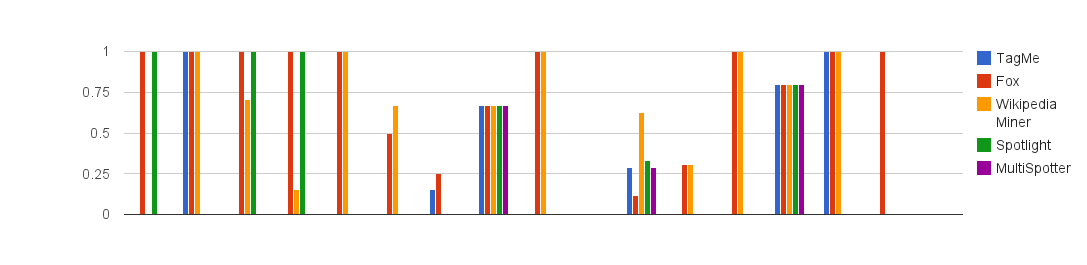
\includegraphics[width=\linewidth]{bars}
%\caption{Entity annotations systems performance with optimal ranking}
%\label{chahawk:fig:spiderOfEntityAnnotators}
%\end{figure}
Our results suggest that HAWK is able to retrieve correct answers with an F-measure of 0.68 using FOX as entity annotation system and assuming an optimal ranking.
Furthermore, the optimal ranker is only able to achieve an F-measure of 0.58 since HAWK can cope better with missing annotation results and is tuned towards retrieving full-text information.
Against intuition, the Union annotator is the worst annotation system. 
Merging all annotation results in queries consisting solely of semantic resources eliminating the possibility to match ontology properties and classes to important parts of the query, e.g., matching the word \texttt{author} to resource rather than to a property prevents HAWK from generating the correct SPARQL query.
Thus, the Union annotator achieves only an F-measure of 0.10.\footnote{Details on this evaluation can be found in the supplement on our project homepage.}


\subsection{Influence of the Ranking Method}
Next, evaluating the effectiveness of the feature-based ranking has to include an in-depth analysis of the contribution of each feature to the overall result.
Thus, we calculated the power set of the set of features and evaluated each feature group using the F-measure reached by the top n queries. 
Figures~\ref{chahawk:fig:ranking_1} and ~\ref{chahawk:fig:ranking_2} show the F-measure@N for all query result sets of size $N$ from all 17 questions. 
%\todo[inline]{What exactly is shown in Figure 4 - i.e. there are F1/Precision/Recall scores for each of the 17 questions the system could answer, but how is the score calculated? I.e. either the systems get the right answer or not? Or is this based on top-N answers? Or based on how many correct answers from all the candidate queries?}
%\begin{minipage}{0.49\textwidth} 
%\centering
\begin{figure}[htb!]
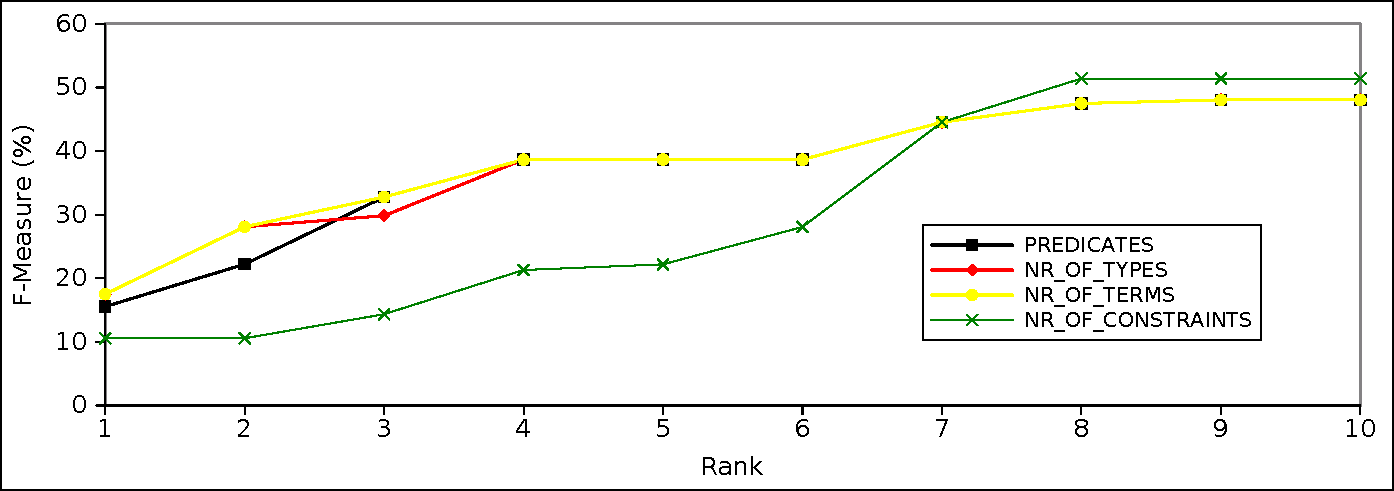
\includegraphics[width=\linewidth]{part_03/ESWC_HAWK/onefeature}
%\captionof{figure}{F-measures on training dataset using $N=[1,\ldots,10]$ and one feature.}
\caption{F-measures on training dataset using $N=[1,\ldots,10]$ and one feature.}
\label{chahawk:fig:ranking_1}
\end{figure}
%\end{minipage}
%\hfill
%\begin{minipage}{0.49\textwidth}
%\centering
\begin{figure}[htb!]
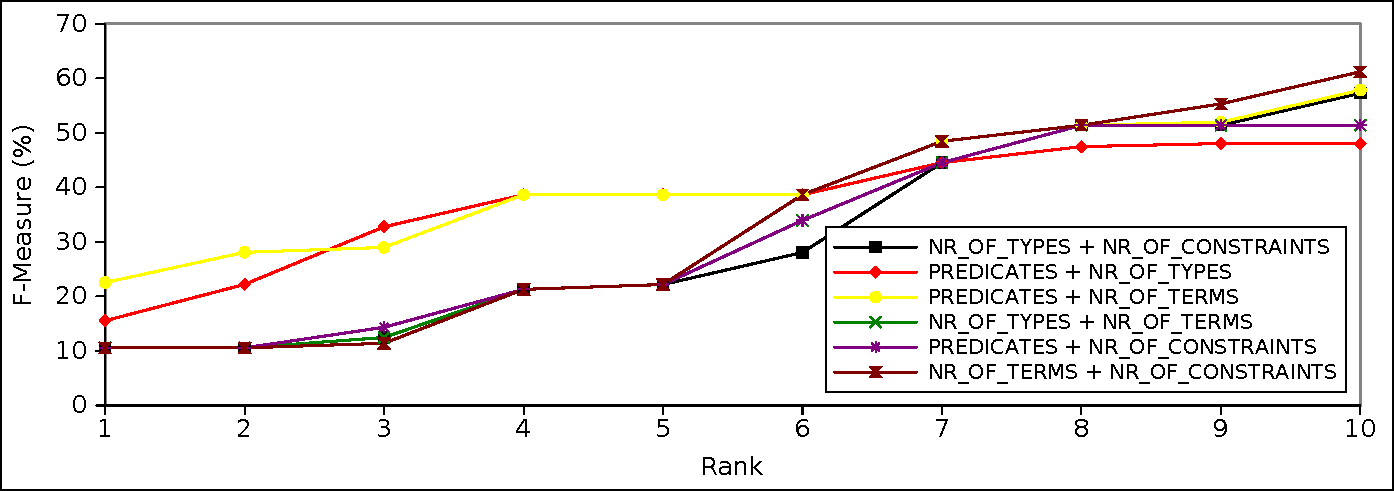
\includegraphics[width=\linewidth]{part_03/ESWC_HAWK/twofeature}
%\captionof{figure}{F-measures on training dataset using $N=[1,\ldots,10]$ and two features.}
\caption{F-measures on training dataset using $N=[1,\ldots,10]$ and two features.}
\label{chahawk:fig:ranking_2}
\end{figure}
%\end{minipage}

%\begin{minipage}{0.49\textwidth} 
%\centering
%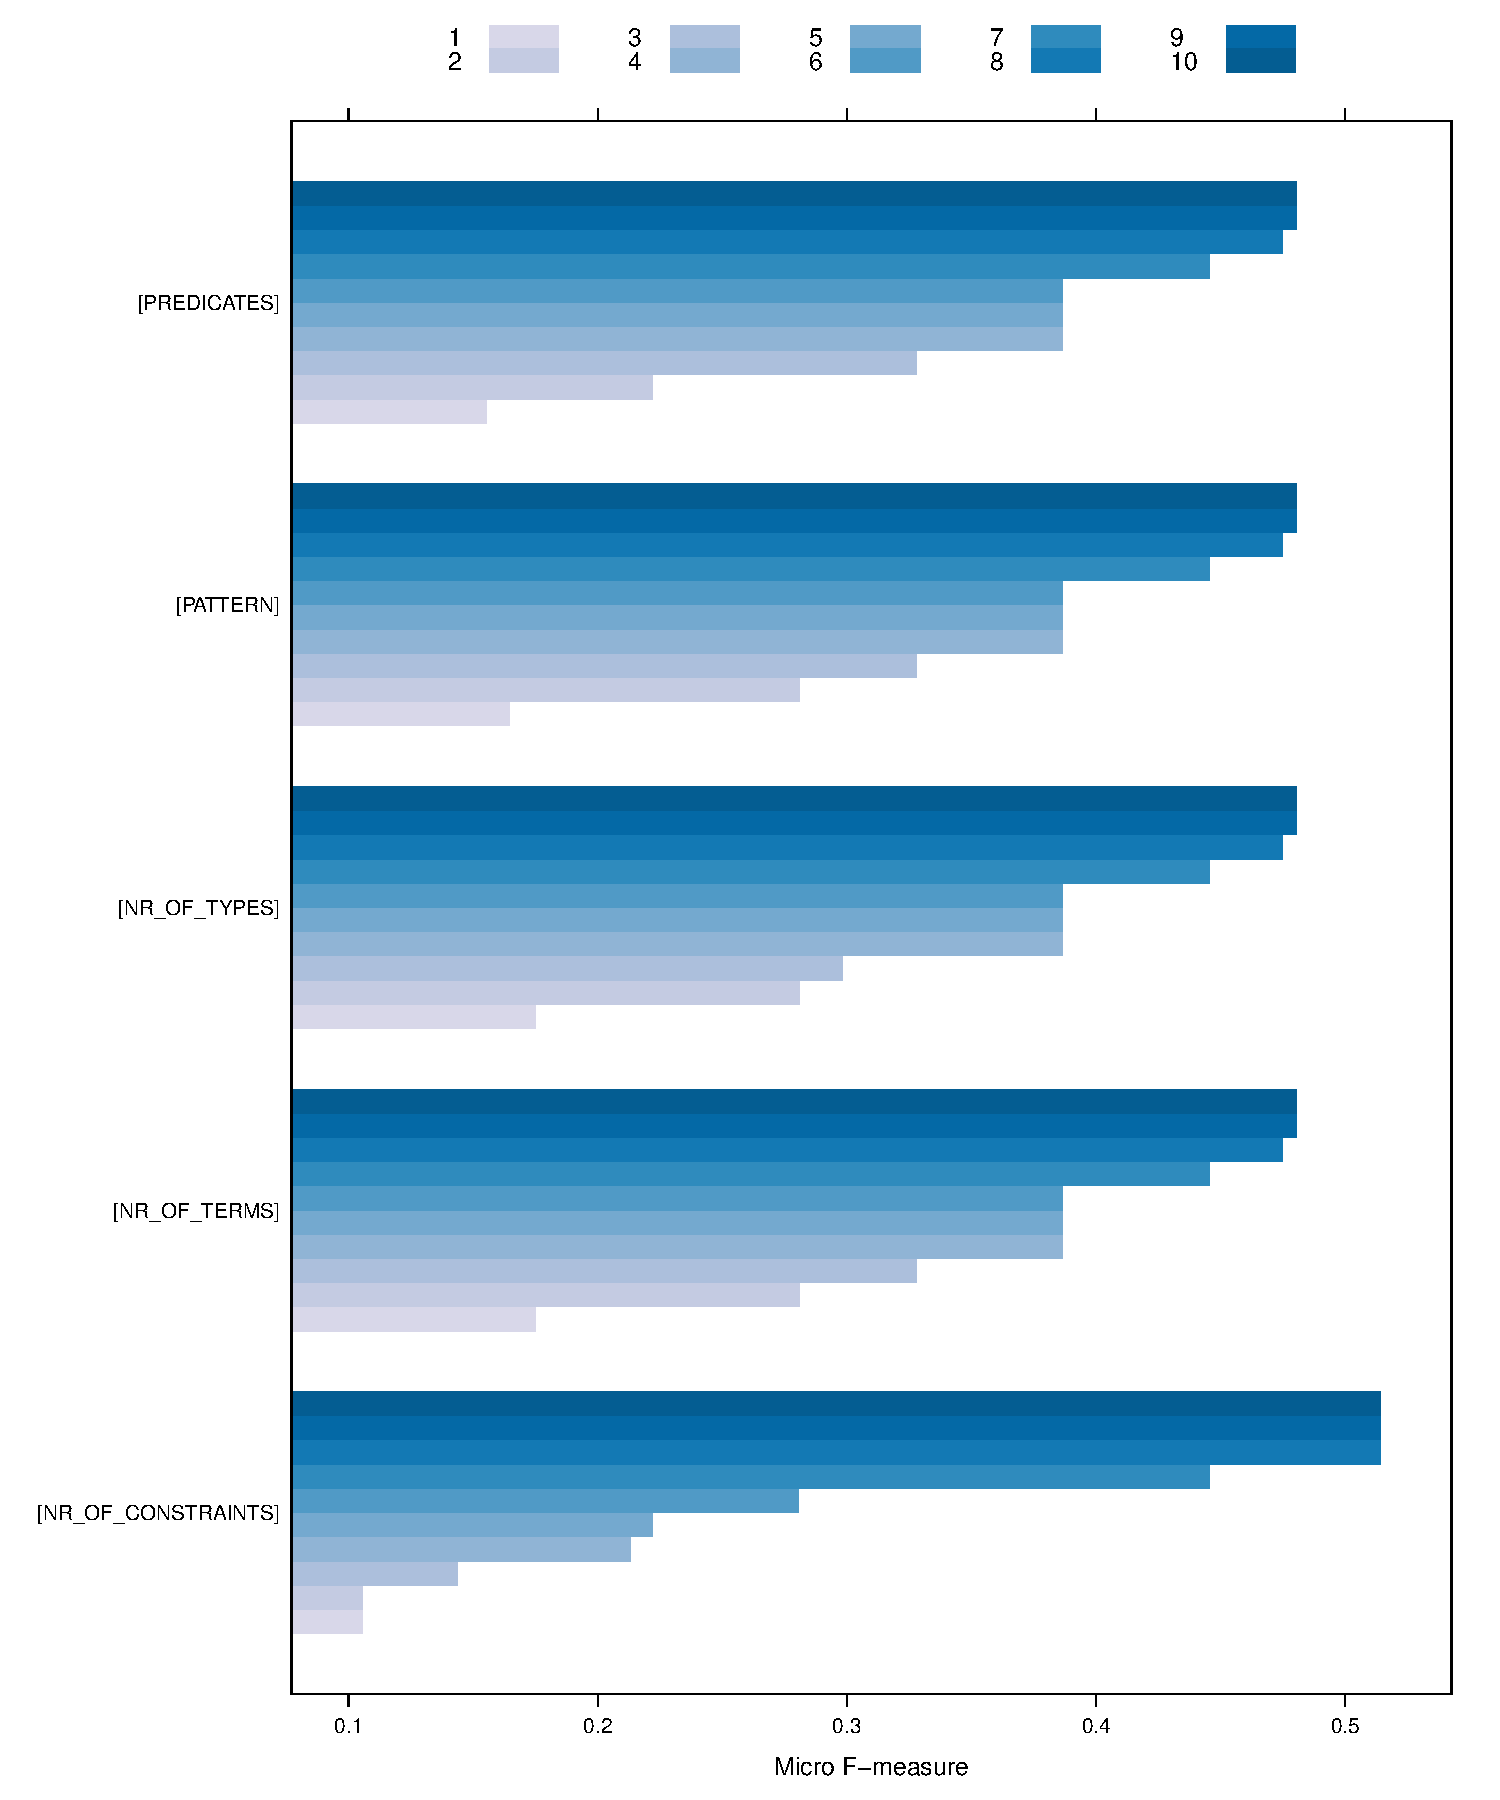
\includegraphics[width=\linewidth]{ranking_1}
%\captionof{figure}{F-measures on training dataset using $N=[1,\ldots,10]$ and one feature.}
%\label{chahawk:fig:ranking_1}
%\end{minipage}
%\hfill
%\begin{minipage}{0.49\textwidth}
%\centering
%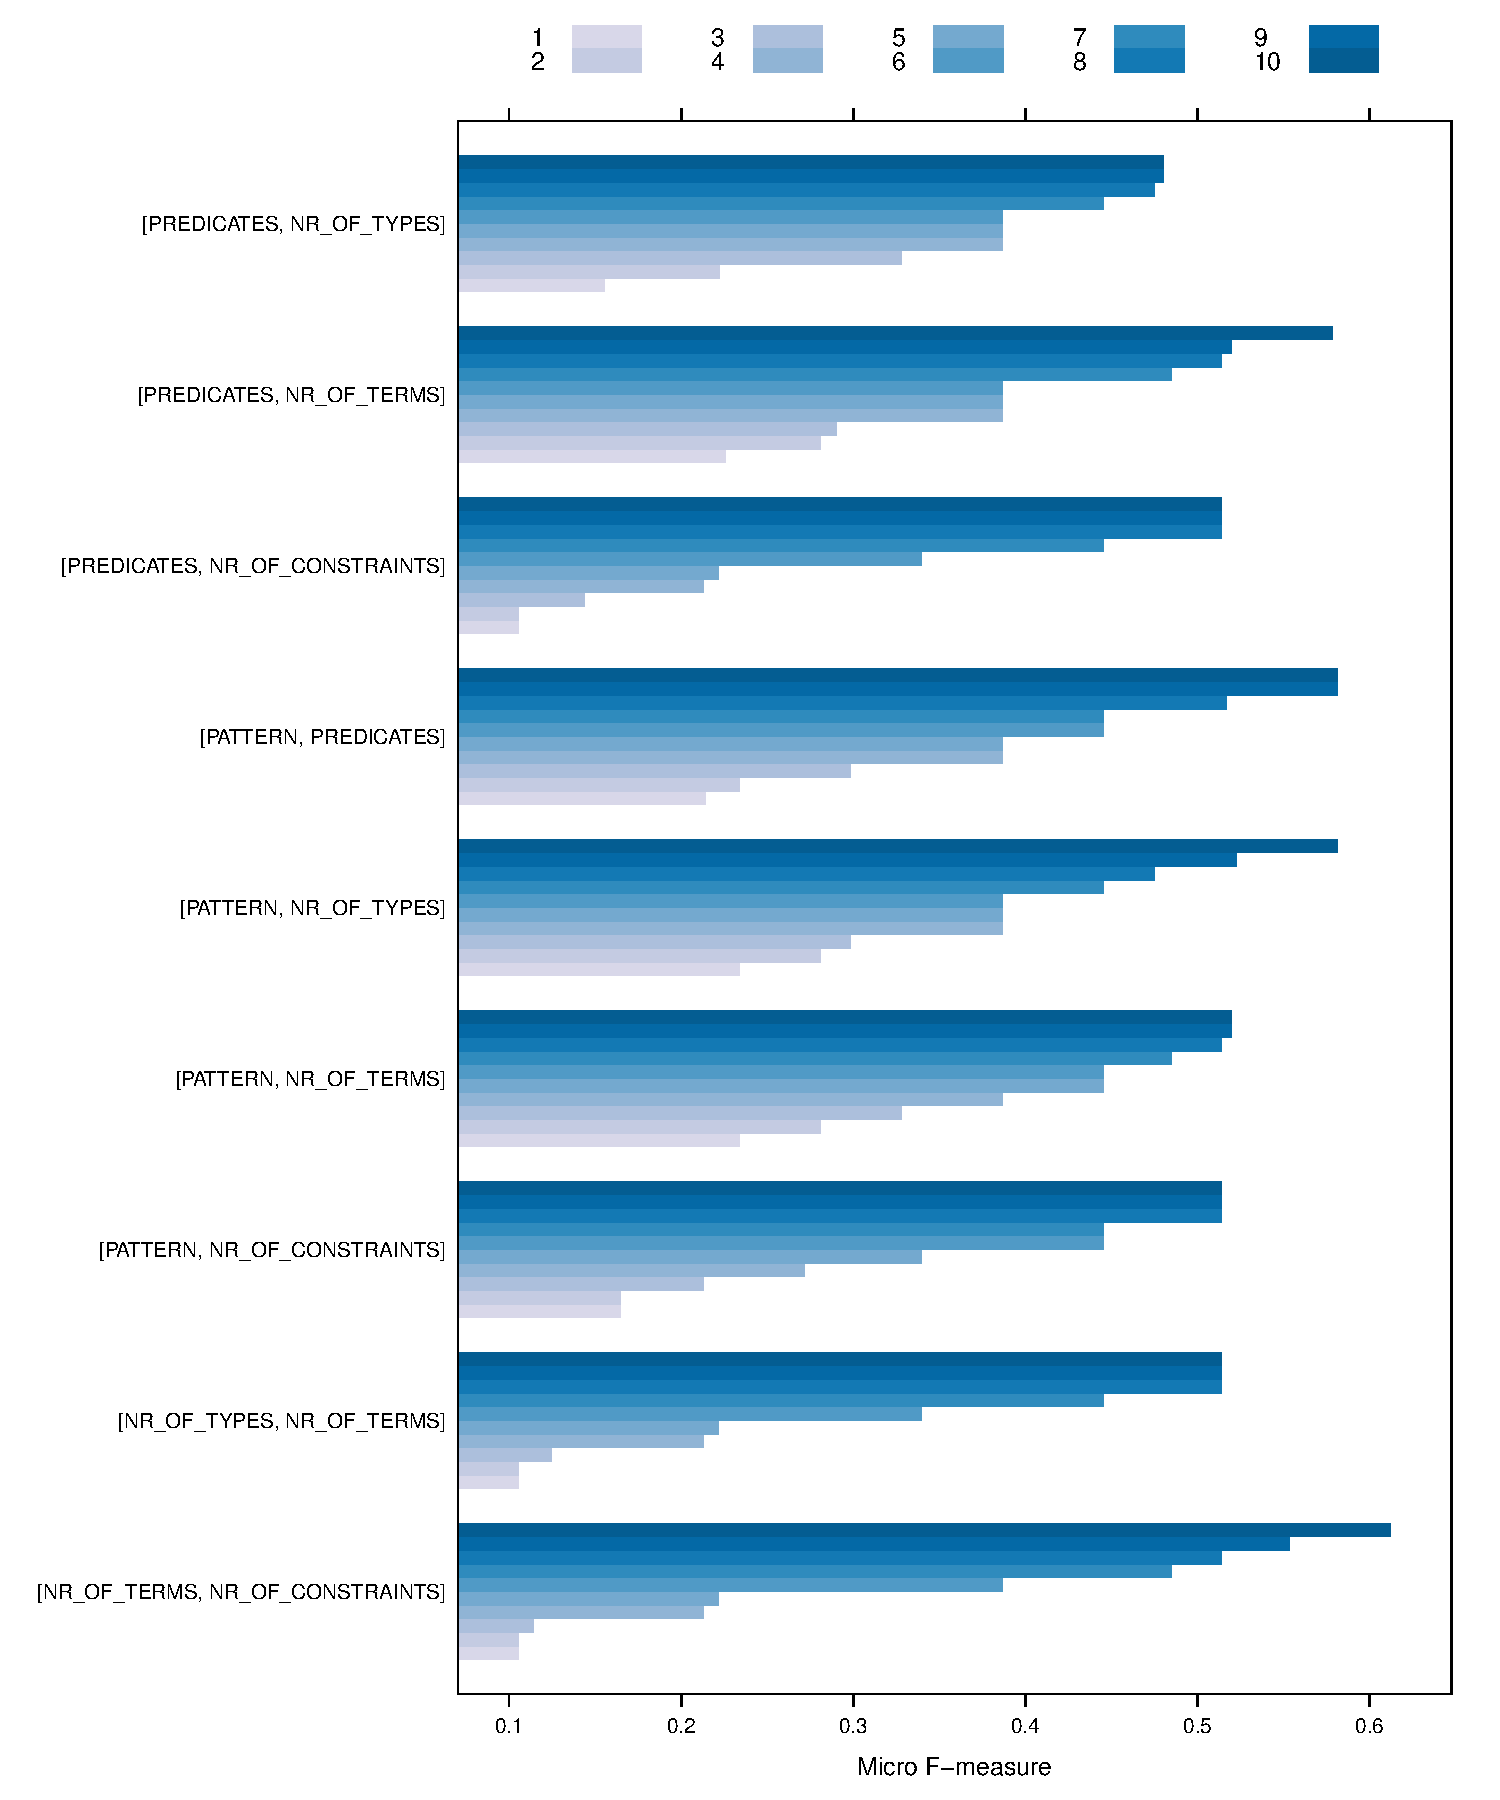
\includegraphics[width=\linewidth]{ranking_2}
%\captionof{figure}{F-measures on training dataset using $N=[1,\ldots,10]$ and two features.}
%\label{chahawk:fig:ranking_2}
%\end{minipage}

%\begin{minipage}{0.49\textwidth} 
%\centering
%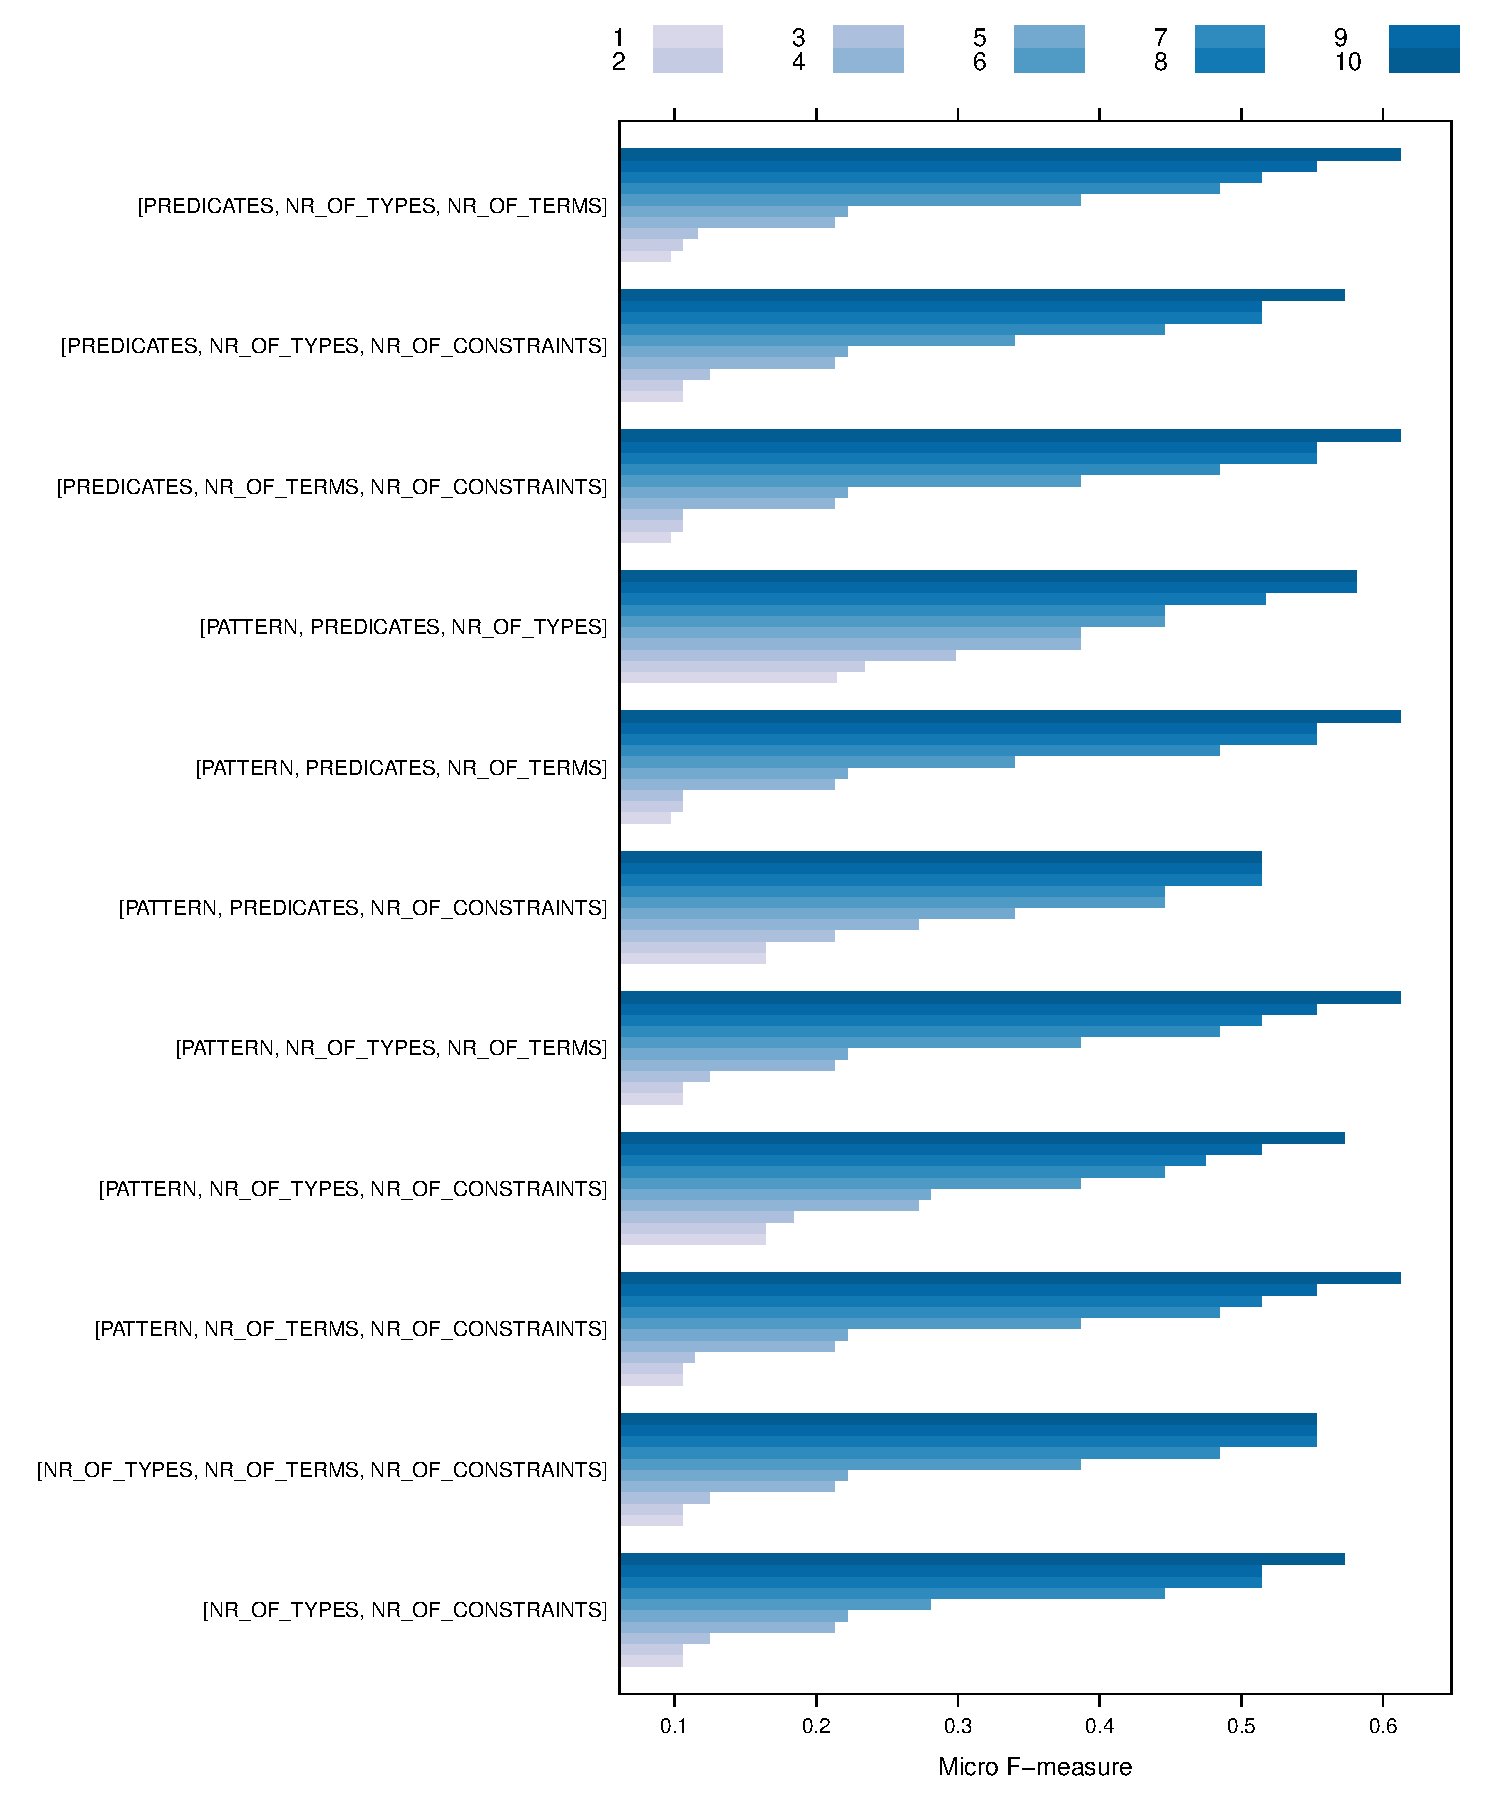
\includegraphics[width=\linewidth]{ranking_3}
%\captionof{figure}{F-measures on training dataset using $N=[1,\ldots,10]$ and three features.}
%\label{chahawk:fig:ranking_3}
%\end{minipage}
%\hfill
%\begin{minipage}{0.49\textwidth}
%\centering
%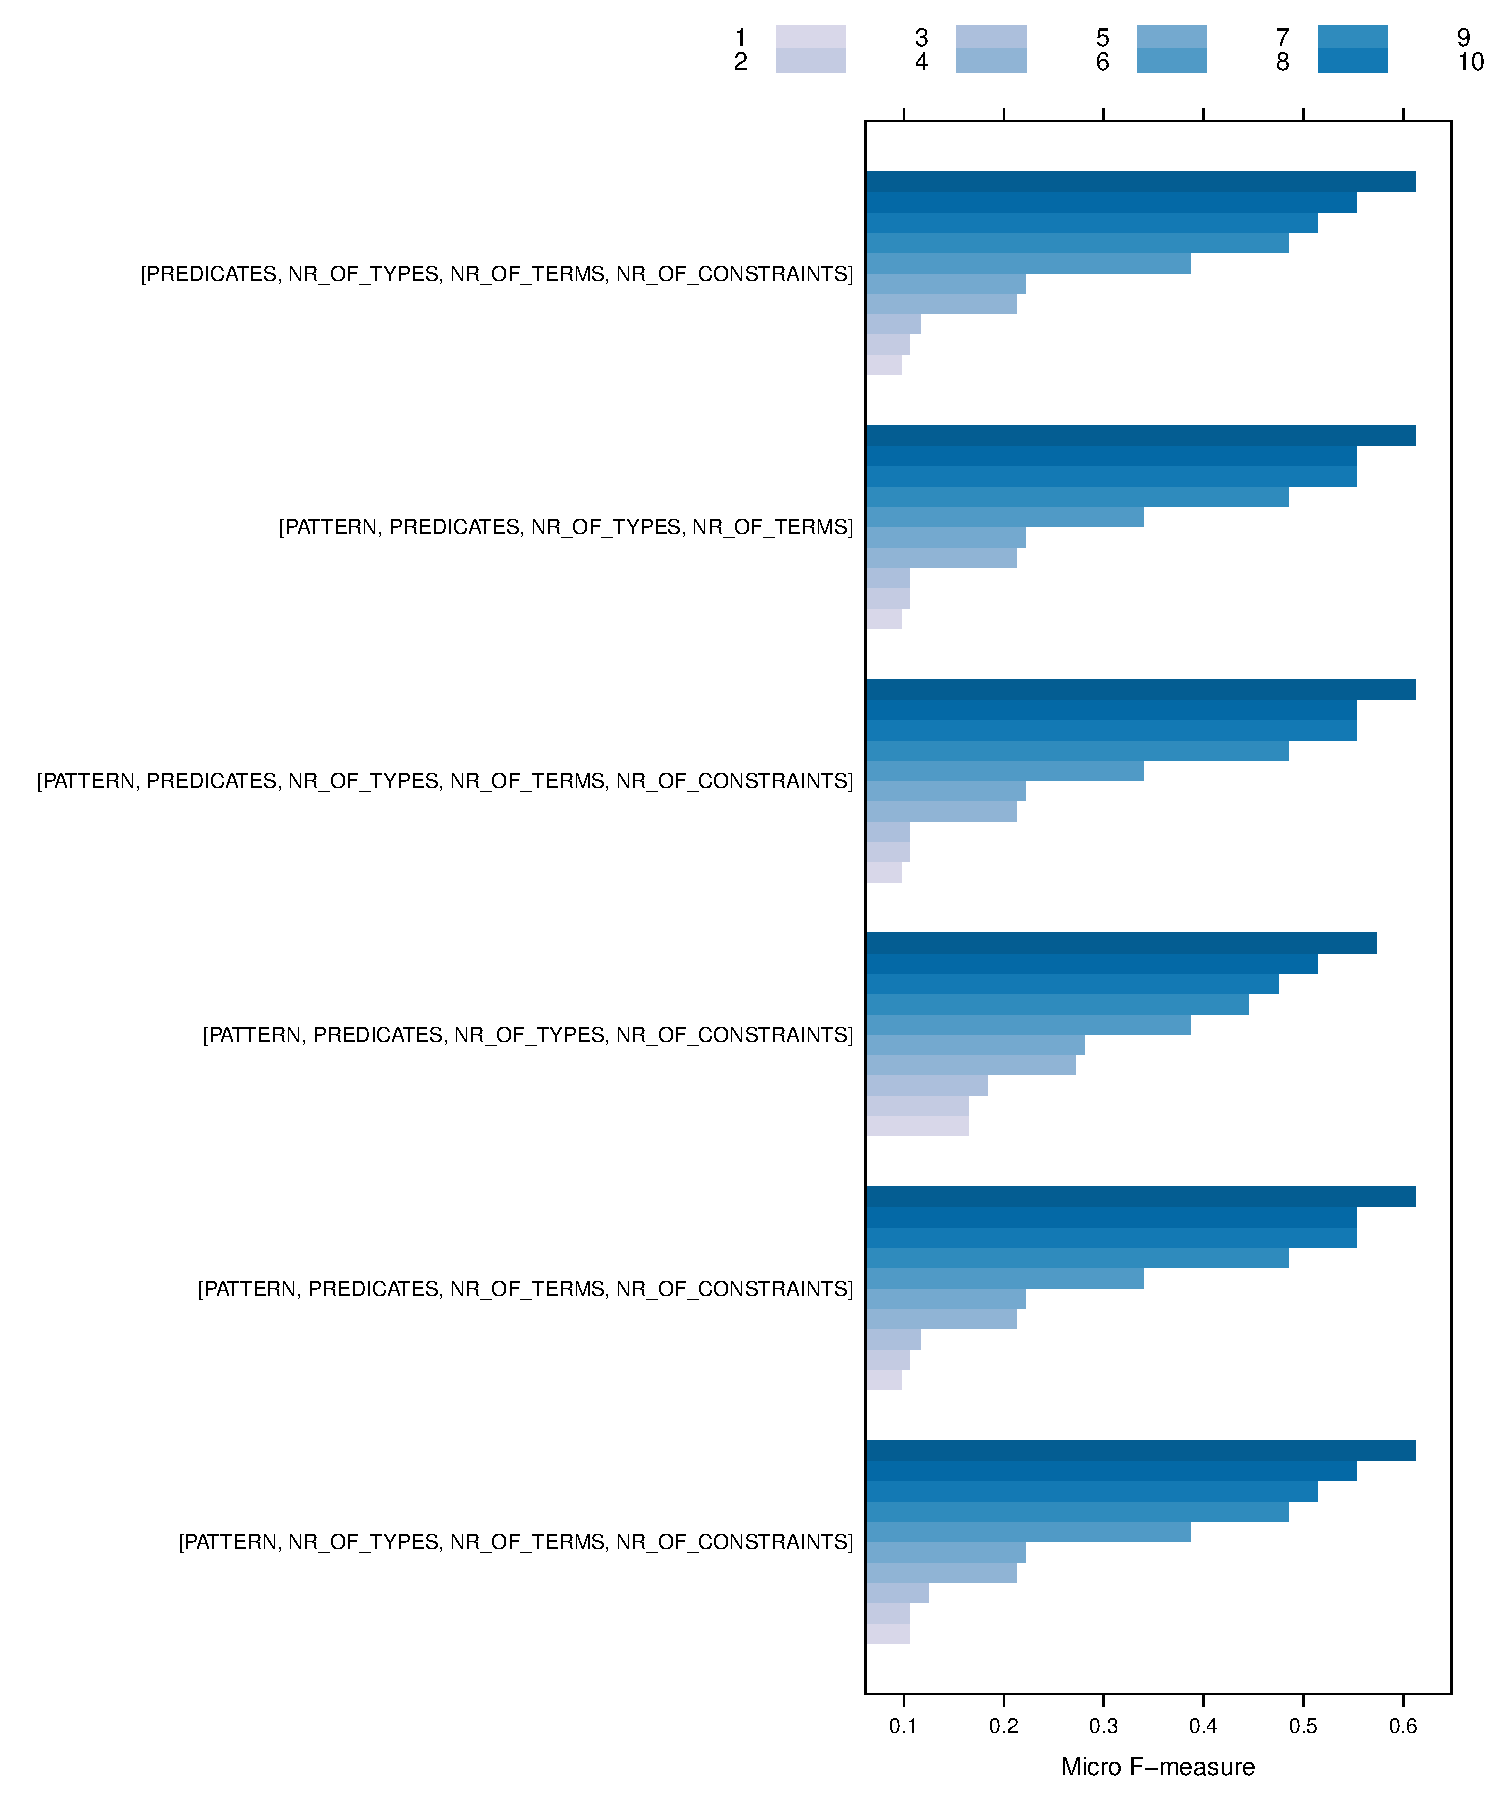
\includegraphics[width=\linewidth]{ranking_45}
%\captionof{figure}{F-measures on training dataset using $N=[1,\ldots,10]$ and using four and five features.}
%\label{chahawk:fig:ranking_45}
%\end{minipage}

Delving deeper into this analysis, we find:
\begin{itemize}
\item Although \textbf{NR\_OF\_TERMS} produces the largest sum of F-measures as a single feature, \textbf{NR\_OF\_CONSTRAINTS} achieves a higher F-measure as soon as $N=7$ due to the larger number of needed constraints with respect to the query length.
\item The highest mass of F-measure reaches the pair \textbf{PREDICATES, NR\_OF\_TERMS} with an F-measure of 0.58 at $N=10$. However, HAWK is able to achieve a higher F-measure of 0.61 at $N=10$ using \textbf{NR\_OF\_TERMS, NR\_OF\_CONSTRAINTS}.
\item We only regard the top-10-ranked queries. The correct queries belonged to the top-n queries as shown in Table~\ref{tab:trainqueries}.
\item The combination of three or all four features does not lead to an improvement. % of the F-measure. 
\end{itemize}

HAWK generates up to 15000 SPARQL queries per question containing more than one query generating the correct answer. 
%\todo[inline]{elaborate}
We consider ranking the resulting SPARQL queries most challenging with respect to the fact that an ideal ranking can lead to F-measures up to 0.72 at $N=1$.
%\todo[inline]{@Axel: does that make sense here: show graph where queries with expected several entities in the answer have LIMIT N against F-measure}

\subsection{Error Analysis}

In the following, we analyze error sources in HAWK based on the training queries failing to reach a higher F-measure.
Table~\ref{tab:trainqueries} shows for each entity search question from the training dataset its evaluation results.
\begin{itemize}
\item \textbf{Entity Annotation: } Queries 1, 11 and 15 cannot be answered by HAWK due to failing entity annotation. None of the tested annotation tools was able to either find the resources  \texttt{Jane\_T.\_Austion} nor \texttt{G8} or \texttt{Los\_Alamos}. 
Without matching entity annotations a full-text search retrieves too many matches for reaching high precision values on limited result set.
\item \textbf{Missing type information:} some of the resources of the gold standard do not have appropriate type information leading to a high amount of queries that need to be ranked correctly.
\item \textbf{Query structure: } Queries like 11 or 15 inherit complex query structures leading to a multitude of interpretations while generating the SPARQL query graph.
\end{itemize}

%% Please add the following required packages to your document preamble:
% \usepackage{booktabs}
% \usepackage[table,xcdraw]{xcolor}
% If you use beamer only pass "xcolor=table" option, i.e. \documentclass[xcolor=table]{beamer}
\begin{table}[htb!]

 \resizebox{\textwidth}{!}{
\begin{tabular}{@{\extracolsep{\fill} } @{}lp{0.55\linewidth}lll@{}}
\toprule
\textbf{ID} & \textbf{Question}                                                                                 & \textbf{F-measure} & \textbf{Precision} & \textbf{Recall} \\ \midrule
\rowcolor[HTML]{FFCCC9} 
1           & Give me the currencies of all G8 countries.                                                       & 0.0                & 0.0                & 0.0             \\
2           & In which city was the assassin of Martin Luther King born?                                        & 1.0                & 1.0                & 1.0             \\
3           & Which anti-apartheid activist graduated from the University of South Africa?                      & 1.0                & 1.0                & 1.0             \\
\rowcolor[HTML]{BBDAFF} 
5           & Which recipients of the Victoria Cross died in the Battle of Arnhem?                              & 0.8                & 0.67               & 1.0             \\
6           & Where did the first man in space die?                                                             & 1.0                & 1.0                & 1.0             \\
\rowcolor[HTML]{BBDAFF} 
8           & Which members of the Wu-Tang Clan took their stage name from a movie?                             & 0.31               & 0.18               & 1.0             \\
\rowcolor[HTML]{BBDAFF} 
9           & Which writers had influenced the philosopher that refused a Nobel Prize?                          & 0.71               & 0.56               & 1.0             \\
\rowcolor[HTML]{FFCCC9} 
11          & Who composed the music for the film that depicts the early life of Jane Austin?                   & 0.0                & 0.0                & 0.0             \\
14          & Which horses did The Long Fellow ride?                                                            & 1.0                & 1.0                & 1.0             \\
\rowcolor[HTML]{9AFF99} 
15          & Of the people that died of radiation in Los Alamos, whose death was an accident?                  & 0.67               & 1.0                & 0.5             \\
\rowcolor[HTML]{BBDAFF} 
16          & Which buildings owned by the crown overlook the North Sea?                                        & 0.25               & 0.14               & 1.0             \\
\rowcolor[HTML]{BBDAFF} 
17          & Which buildings in art deco style did Shreve, Lamb and Harmon design?                             & 0.5                & 0.33               & 1.0             \\
18          & Which birds are protected under the National Parks and Wildlife Act?                              & 1.0                & 1.0                & 1.0             \\
19          & Which country did the first known photographer of snowflakes come from?                           & 1.0                & 1.0                & 1.0             \\
20          & List all the battles fought by the lover of Cleopatra.                                            & 1.0                & 1.0                & 1.0             \\
22          & Which actress starring in the TV series Friends owns the production company Coquette Productions? & 1.0                & 1.0                & 1.0             \\
23          & Dakar is the capital of which country member of the African Union?                                & 1.0                & 1.0                & 1.0             \\ \bottomrule
\end{tabular}}
\caption[QALD 4 training set performance.]{Micro measures: Precision=0.70 Recall=0.85 F-measure=0.72 at 17 queries from QALD 4 training set. Red indicates inability to generate correct query, Blue indicates missing precision and green missing recall.}
\label{tab:trainqueries}

\end{table}